\documentclass{article}
\usepackage{tikz}
\begin{document}
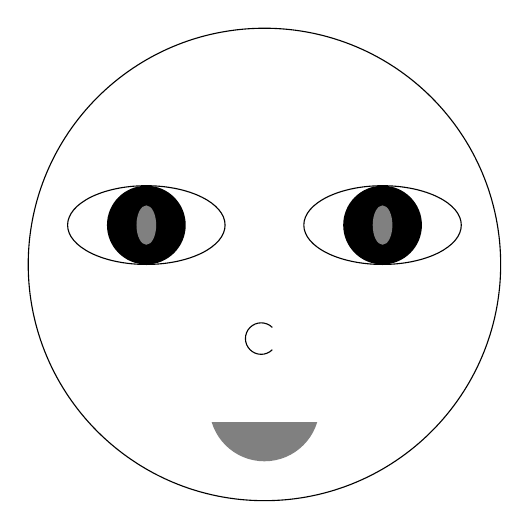
\begin{tikzpicture}
\path (0cm,0cm) coordinate(O);
\draw (O) circle(3cm);
\draw (O)++(0.1cm,-0.8cm) arc(45:315:0.2cm);
\path ++(-1.5cm,0.5cm) coordinate (P1) ++(3cm,0cm) coordinate (P2);
\foreach \i in {1,2}{
\draw (P\i) ellipse(1cm and 0.5cm);
\fill[black] (P\i) circle (0.5cm);
\fill[gray] (P\i) ellipse (0.125cm and 0.25cm);
}
\begin{scope}
\clip (O)++(0,-1.8cm) circle (0.7cm);
\fill[color=gray](-3cm,-3cm) rectangle (2cm,-2cm);
\end{scope}
\end{tikzpicture}
\end{document}